% !TeX root = ../DistributedConsensus.tex
% !TeX spellcheck = en_GB
\chapter{Background}\label{chap:background}
	\section{Dynamic Condition Response Graphs}\label{sec:background:dcrgraphs}
	A Dynamic Condition Response Graph is a declarative, event-based process model. Instead of using sequences of state transitions like imperative process languages, declarative process languages uses sets of constraints to model the possible transitions in the process (hereafter \textit{workflow}). A benefit of DCR graphs is that they allow finite specifications of infinite behaviour.

%	Since events in a DCR graphs are distributed and no algorithm for finding the order of execution currently exists, DCR graphs are well suited for developing an algorithm for determining history. 
%	Furthermore DCR graphs specify several types of directed edges in the graph, which provide useful information for determining order of execution.
	
	\newpar A DCR graph is in \cite{hildebrandt2011declarative} defined as a tuple $(E, M, Act, $\condition$, $\response$, \pm, l)$ where
	\begin{itemize}
		\item $E$ is the set of events
		\item $M$ is the marking, the state of the workflow. The marking is a triple containing three sets of events. The first set contains the events that have previously been executed. The second set contains the events that are required to be executed or excluded. These are called the pending responses. The last set contains the events which are currently included.
		\item $Act$ is the set of \textit{actions}. That is, a representation of what happens in the workflow when a given event is executed.
		\item \condition (conditions) is a relation, which for all pairs of events which are present in the relation, means that the first event must be either excluded or executed for the second event to be executable.
		\item \response (responses) is a relation, which for all pairs of events which are present in the relation, means that after the first event has been executed the second event must either be executed or excluded at some point for the workflow to be in an accepting state.
		\item $\pm$ defines the dynamic inclusion and exclusion of events. This partial function is a triple of two events and symbol defining whether the execution of the first event should result in an exclusion or inclusion of the second event. It is possible for an event to exclude itself, but one event cannot both include and exclude another.
		\item $l$ is the labelling function, assigning an \textit{action} to each event.
	\end{itemize}
		
	Furthermore the article defines a distributed DCR graph as a DCR graph with a set of roles, a set of principals, and a mapping function that assigns roles to principals and actions. This assignment means that if principal $P$ is assigned role $R$, and action $A$ is assigned $R$, then $P$ can execute $A$.
		
	\newpar
	Events can be safely distributed by defining \textit{projections} and \textit{compositions} of DCR graphs. This is described in \cite{hildebrandt2011safe}. This idea of distributing events between multiple processes in a distributed system is used in the DCR graph implementation used for this project. This implementation is further described in \autoref{sec:background:implementation}. 
    
	\newpar 
	In \cite{debois2015concurrency}, Debois et al. describes the procedure for executing distributed events using a locking mechanism to ensure serial equivalence:
	
	\begin{quotation}
		``\textit{The procedure for executing an event, in detail, is as follows. A component
		wishing to execute an event $e$ must first request\footnote{All components request locks in the same fixed order to prevent deadlocks.} and receive locks on all (local
		and remote) events that are in conflict (i.e., not independent) with $e$ (thus, in
		particular, on itself). It then queries the state of remote events to determine if
		$e$ is currently executable. If it is, it instructs remote events affected by firing $e$
		to change state accordingly. Finally, it releases all locks.}''
	\end{quotation}
	
	 \noindent Furthermore, Debois et al. states in \cite{debois2015concurrency} that for two events to have concurrent executions the events must be independent, that is the events must be effect and cause-orthogonal. In the article effect-orthogonality is described as
	\begin{itemize}
		\item ``no event included by $e$ is excluded by $f$ and vice versa, and''
		\item ``$e$ requires a response from some $g$ $iff$ $f$ does.''
	\end{itemize}
	
	\noindent and cause-orthogonality is described as
	\begin{itemize}
		\item ``neither event is a condition for the other,''
		\item ``neither event includes or excludes the other, and''
		\item ``neither event includes or excludes a condition of the other.''
	\end{itemize}

	\section{Distributed Systems}
		Distributed systems is an area of computer science which focuses on the concepts, problems and design of computer systems where message transmission among processes are not negligible compared to the time between events in a single process\cite{Lamport:1978:TCO:359545.359563}. Traditionally these systems are distributed on computers in a network.
		
		\subsection{Serial Equivalence}
		Operations performed by two concurrent processes are serially equivalent if the resulting system state is the same as if any one of the processes' operations happened first, followed by the other. In distributed systems this term is used for transactions across machines in a network and is especially important since message passing over network connections introduce inconsistent and unpredictable delays. Therefore multiple messages can arrive at different times, even if they were supposed to happen in sequence. An example of a serial equivalent interleaving of two transactions is shown in \autoref{fig:background:serial-equivalence}. Common implementations of achieving serial equivalence in distributed systems include locking and optimistic concurrency control. In \cite{Coulouris:2011:DSC:2029110:chapter16} these concepts are explored in depth.
		
		\begin{figure}[H]
		\centering
		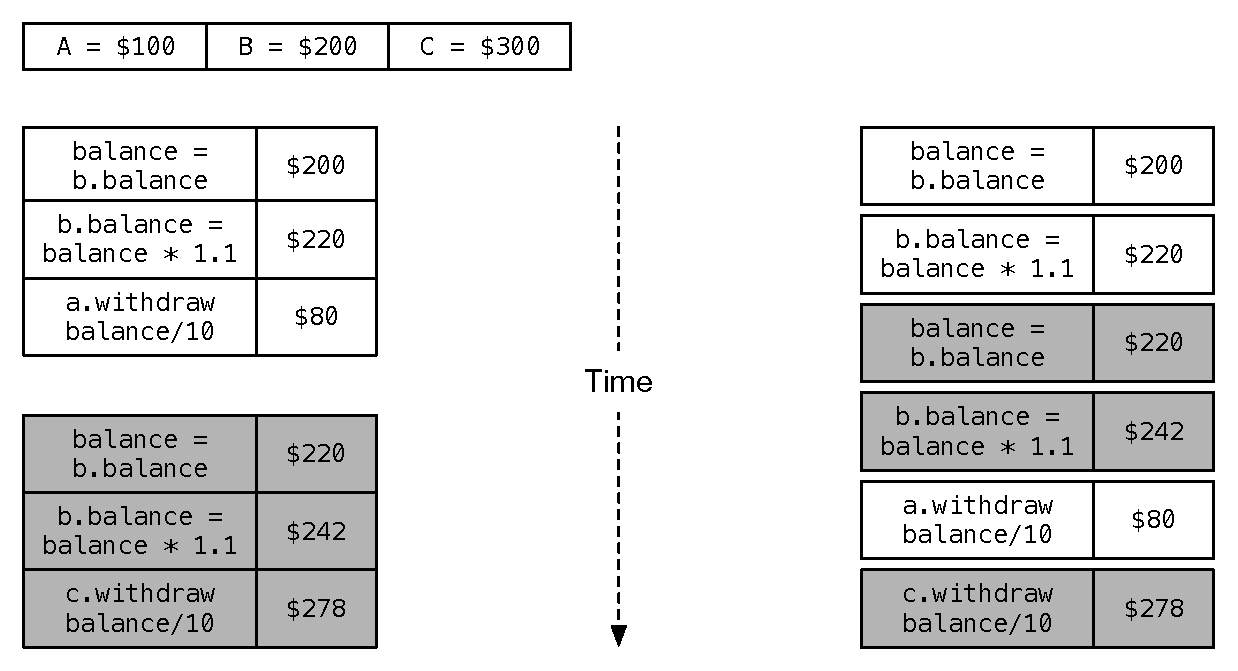
\includegraphics[width=\textwidth]{2background/images/serial-equivalence.pdf}
		\caption{Two transactions executed in sequence and a serially equivalent interleaving.}
		\label{fig:background:serial-equivalence}
		\end{figure}
		
		\subsection{Ordering of Events}\label{subsec:orderingofevents}
		In \cite{Lamport:1978:TCO:359545.359563} Leslie Lamport examines and describes the ordering of events in distributed systems (not to be confused with DCR events) based on their occurrence in time.

		\newpar In set theory a strict total order is an order that is \textit{antisymmetric}, that is if $a \leq b$ and $b \leq a$ then $a = b$, \textit{transitive}, that is if $a \leq b$ and $b \leq c$ then $a \leq c$, \textit{total}, that is $a \leq b$ or $b \leq a$, in addition to being \textit{irreflexive}, that is $a \not< a$. A \textit{strict partial order} is similar to a \textit{strict total order}, but does not have the \textit{totality} property.
        
		These orders can be described with two examples, using a subset of the natural numbers, $\{1, 2, 3, 4, 5, 6\}$ referred to as $N$. An example of a strict total order is $N$ ordered by the less than ($<$) relation. An example of a strict partial order is $N$ ordered by the proper divisors. An illustration of these two orders can be found seen on \autoref{fig:background:strict-partial} and \autoref{fig:background:strict-total}.
	
		\begin{figure}[H]
		\centering
		\begin{minipage}{0.45\textwidth}
			\centering
			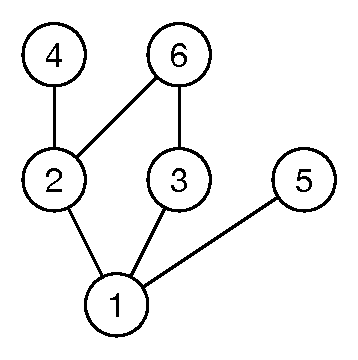
\includegraphics[height=\textheight/5]{2background/images/strict-partial.pdf}
		\caption{The strict partial order of $N$ ordered by the proper divisors. $A$ $\rightarrow$ $B$ denotes $A$ is a proper divisor $B$.}
		\label{fig:background:strict-partial}
		\end{minipage}\hfill
		\begin{minipage}{0.45\textwidth}
			\centering
			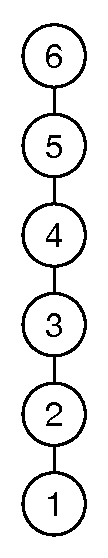
\includegraphics[height=\textheight/5]{2background/images/strict-total.pdf}
		\caption{The strict total order of $N$ ordered by the less than ($<$) relation.}
		\label{fig:background:strict-total}
		\end{minipage}
		\end{figure}
		
		\newpar Lamport introduces so-called \textit{logical clocks}, which are simple timestamps that enable determining the order of events in a distributed system. The clocks are \textit{logical} because they do not represent \textit{physical} time, since synchronising physical time in a distributed system is a non-trivial task. A logical clock is a simple counter that is incremented for each event happening in a process. 
		
		When a process receives a message, the counter must be set to a higher value than both the received timestamp, as well as the local clock. This also implies that each message must include the timestamp of the sending event. This is illustrated in \autoref{fig:background:lamport-timestamps}
		
		\begin{figure}[H]
		\centering
		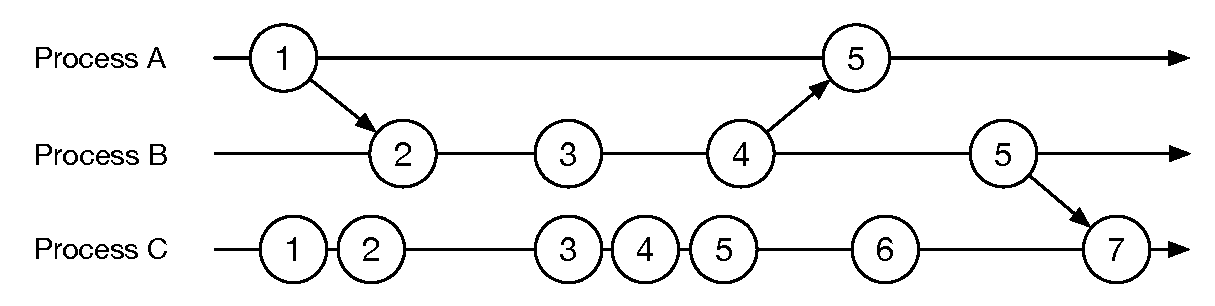
\includegraphics[width=\textwidth]{2background/images/lamport-timestamps.pdf}
		\caption{Three processes exchanging messages and setting their local timestamps accordingly.}
		\label{fig:background:lamport-timestamps}
		\end{figure}
		
		\newpar Lamport argues that if a given system is not distributed it is possible to create a history of events where the ordering is total, since it is possible for one process to use a logical clock to find out which event happened before another. In a distributed system however, this global ordering is not possible since events have independent locical clocks that are set to the same timestamp.
		
		\newpar Lamport describes these relations between events with the symbol $\rightarrow$ such that if $event$ $a$ happens before $event$ $b$ then $a \rightarrow b$. These relations can be created based on three cases:
        
        \begin{enumerate}
        	\item If $event$ $a$ and $b$ happened on the same process and $a$ happened before $b$ measured with the local logical clock then $a \rightarrow b$.
            \item If process $i$ sends a message to process $j$ and $event$ $a$ is the event which initiates the sending and $event$ $b$ is the recieving of the message then $a \rightarrow b$.
            \item If $a \rightarrow b$ and $b \rightarrow c$ then $a \rightarrow c$, that is, it is transitive.
        \end{enumerate}
        
        \noindent If no relation exists between any event $a$ and $b$, the events are \textit{concurrent} and logically occur at the same time, even though this might not be the case physically. Lamport therefore argues that it is only possible to find a strict partial order of events in distributed systems.
		
		\subsection{Consensus}
		Traditionally consensus in distributed systems is the activity of reaching agreement among the participants in the system on a proposed value. The consensus problem has the following three requirements as stated in \cite{Coulouris:2011:DSC:2029110:chapter15}:
		\begin{itemize}
			\item Termination: Eventually each correct process sets its decision variable.
			\item Agreement: The decision values of all correct processes are the same.
			\item Integrity: If the correct processes all proposed the same value, then any correct process in the decided state has chosen that value.
		\end{itemize}
		
		\newpar Such problems are often achieved by using an consensus algorithm such as Paxos\cite{Lamport:1998:PP:279227.279229} and Raft \cite{Raft:Ongaro:184040}.
		
		Assumptions about the distributed system are made for both Paxos and Raft, namely, processes operate at an arbitrary speed, may experience failures, may recover after a crash by storing their state, and do not collude, lie or attempt to subvert the protocol; in short, Byzantine failures do not occur.
		
		In our problem domain processes may operate at an arbitrary speed and \textit{may} collude, lie or attempt to subvert the protocol; Byzantine failures \textit{do} occur. Therefore it is not possible to use Paxos or Raft for this project. 
		 
		\newpar The \textit{Byzantine generals problem} is a case of the consensus problem. Instead of having multiple proposers, the commander is introduced. Byzantine failures are allowed and handled by signing messages. Also, each process needs to be connected to all other processes and there is a limit of a third malicious processes that can exist in the system. It has been proven that the Byzantine generals problem cannot be solved for a system with only two processes. \cite{Lamport:1982:BGP:357172.357176}
        
	\section{Directed Graphs}
		A \textit{directed graph} is a data structure which consists of \textit{nodes} connected by \textit{edges}. In directed graphs an edge is an ordered pair of nodes, where the first element is the start node and the second is the end node. When traversing the graph, it is only possible to traverse edges from their start node to their end node. There exists a \textit{path} from a node to another if it is possible through one or more edges in succession to get from the first to the second node.
	
		For a given node, the \textit{reachability} is the set of all the nodes there exists a path to. For a graph to be \textit{acyclic} any node in the graph must not have a path to itself. 
	
		The subgraph of a given graph with the same reachability of each node, but with as few edges as possible, is called the \textit{minimum equivalent graph}.
	
		A \textit{topological order} of a directed graph is a total ordering of the nodes, such that for every edge $a,b$ from node $a$ to $b$, $a$ comes before $b$.
		
		\newpar All of these topics are described further in \cite{sedgewick2011algorithms}.
		
	\section{Distributed DCR implementation}\label{sec:background:implementation}
		We have based the implementation of this project on the work done during our second year project.\footnote{For an in depth description of the original implementation the project including a report can be found at \url{https://github.com/andersfischernielsen/FlowIT-Second-Year-Project/}.}
		
		\newpar From the requirements of the second year project:
		
		\begin{quotation}
			\noindent``\textit{The goal is to develop a functioning and correct, web-service based distributed workflow system that can support distributed coordination of workflows provided by the external and possibly international customers, and reconfigured if the workflow changes.}''
		\end{quotation}
		
		\newpar At the time of implementation, only \textit{condition}, \textit{response}, \textit{inclusion}, and \textit{exclusion} relations were required, even though other relations exist, such as the \textit{milestone} and \textit{spawn} relations. 
		
		\newpar In order to fulfil the requirements we separated the project into smaller components:
		
		\begin{itemize}
			\item An event \textit{peer}
			\item A central \textit{server}
			\item A \textit{client}
			\item A parser and uploader to set up the workflows
		\end{itemize}
		
		\newpar An event peer can contain zero or more DCR events. For each of these events, the peer persists information about the event. This information consists of an ID, a name to show in the client in addition to the state of the event which is represented as boolean values for include, pending, and execute. This corresponds to the marking of the projection of a DCR graph where only a single event is chosen as projection parameter. The relations of an event are also stored. Furthermore the initial values of the state are stored in order to be able to restore the workflow to the initial state.
		
		As mentioned above and as opposed to the definition of DCR graphs in \cite{hildebrandt2011declarative} the states of workflows are not saved as markings. Instead the event peer saves the state of each of the events it hosts.
		
		\newpar In order to achieve serial equivalence when executing, a locking strategy has been used because of its simplicity and because performance was not a priority for the project. The system executes events using the procedure from \cite{debois2015concurrency} as quoted in \autoref{sec:background:dcrgraphs}. In order to prevent deadlocks, the order of obtaining locks has been defined inside a workflow. Locks are acquired according to alphabetical order of the IDs of events.
		
		\newpar The central server contains information about workflows and the events that take part in the workflow. Each workflow is identified by an ID, that is chosen when creating the workflow. For each event in a workflow the ID of the event as well as the address of the event peer hosting that event is stored. The server also contains information about users and the roles they are operating with.
		
		\newpar In the client, when a user logs in, the server sends information about which roles the user has access to in the workflows he is connected to. The client can then filter the events of a chosen workflow, so the user only sees events where he or she has the right to execute.
		
		For each accessible event in a workflow, the client shows the name and state of the event. Furthermore, a button used to execute an event exists, which is deactivated if the event is not executable. The client also allows the user to get an overview of what happened in a given workflow. This feature was called "history", but was implemented by ordering each log entry by physical time. This history feature has obviously been replaced with the outcome of this project.
		
		\newpar The parser is a tool developed to make it easier to upload workflows created on DCRGraphs.net\footnote{\url{http://dcrgraphs.net}} into the system.
		
		\subsection{Changes to the original implementation}
			When starting this project, we discovered a few mistakes in the original implementation. Most importantly, conditions were checked before locking the target events, which could mean that this conditioning event could change its state and therefore change whether or not the condition was fulfilled, before the locks on other events were obtained.
            
            Furthermore the aforementioned history implementation has been removed and the parser is now included in the main client project.
            
            \newpar Increasing timestamps for messages received and sent between events are also implemented in ordert to use Lamport timestamps. Timestamps between events should always increase, which means that an event will reject a message with a timestamp lower than the previous timestamp it has received from another event.
            
            \newpar In order to store any kind of information on an event, it must be locked. Furthermore, information about locks are not stored on events.

			\newpar In the aforementioned report, the user guide points to certain URLs that should contain the web services of the system. These web services are no longer running.